\documentclass[10pt]{article}
\usepackage[margin=0.75in]{geometry}
\usepackage[T1]{fontenc}
\usepackage[utf8]{inputenc}
\usepackage{lmodern}
\usepackage{microtype}
\usepackage{booktabs}
\usepackage{amsmath}
\usepackage{graphicx}
\usepackage{hyperref}
\usepackage{xcolor}
\title{TX4 Blind Portfolio Prediction and Contextual Return}
\author{TX4 confirmatory campaign}
\date{14 September 2026}
\begin{document}
\maketitle
\begin{abstract}
A frozen IEEE-39 phasor-domain model contains a four-bus SG-to-GFL portfolio
that is unstable while all fifteen proper subsets are stable. A reusable
all-SG network kernel and four local replacement models predicted this V4
verdict before full-order reveal (16/16, zero false-safe). A contextual
return reaches unity at the same controller boundary, and nonlinear
phasor-domain TDS preserves the ordering. The result is deliberately scoped:
a 512-portfolio V9 benchmark gives 77.15 percent accuracy with 116 false-safe
cases, the reduced method is slower, and the reduced boundary run was
executed after reveal. The appropriate conclusion is CASE B.
\end{abstract}
\section{Executive verdict}
H4=\{30,33,35,37\} is the minimal dynamically unstable portfolio at frozen
P4. The numerical record is delivered with scripts, tables, raw traces,
hashes, figures, and negative results. No universal or probabilistic
generalization is claimed.

\section{Scientific question}
The test is whether one reusable network kernel plus local SG-to-GFL device
substitutions can predict a finite incompatible portfolio and explain it with
an exact contextual return. V4 passes; V9 limits the scope.

\section{Prior evidence and negative lessons}
The frozen TX4 record and prior PowerDynamics/CDW negatives are read-only.
This campaign did not rescue those lines or modify the frozen manuscript.

\section{Frozen TX4 model}
The IEEE-39 phasor-domain DAE uses frozen synchronous-machine, AVR, and
ten-state custom GFL semantics. P4 is
$(g,k,t,h)=(0.03625,1.425,1.5,1)$. The critical positive-frequency band is
0.3--1.5 Hz. No new controller, governor, limits, EMT interface, or network
model was added.

\section{Blind-prediction firewall}
Before reveal, the code built one all-SG $T_0/K(s)$ and local $\Delta Y_i(s)$
library and enumerated V4 and V9. It did not load FC01, PCV02, FC10, H,
kappa, or historical boundary tables. Prediction files were hashed and
committed before reveal. The firewall is in
\texttt{docs/TX4\_BLIND\_FIREWALL.md}.

\section{Baseline kernel and local models}
For portfolio $S$, the audited construction is
$K=E^TT_0^{-1}E$, $M_S=D_SK_{SS}$, and
$Q_S=(I+D_SK_d)^{-1}D_SK_o$. Local models are equilibrium-matched and reused
without post-reveal fitting.

\section{Exact reduced closure}
The root search used the frozen band, deterministic grids, fixed seeds, root
refinement, and a local-factor floor. The factorization is an exact
determinant representation under regularity assumptions; it is not an
away-from-root approximation to the full spectral abscissa.

\section{Blind V4 prediction}
The reduced prediction found H4 exactly. Full-order reveal produced 15 stable
and one unstable case. Accuracy was 16/16, false-safe 0, false-unstable 0,
H exact, and kappa exact at 4. H4 reduced root:
$\operatorname{Re}(s)=0.12700633761\,{\rm s}^{-1}$ and 0.62227967095 Hz.
Full order: $+0.12700646714\,{\rm s}^{-1}$ and 0.62227966958 Hz.

\begin{figure}[ht]
\centering
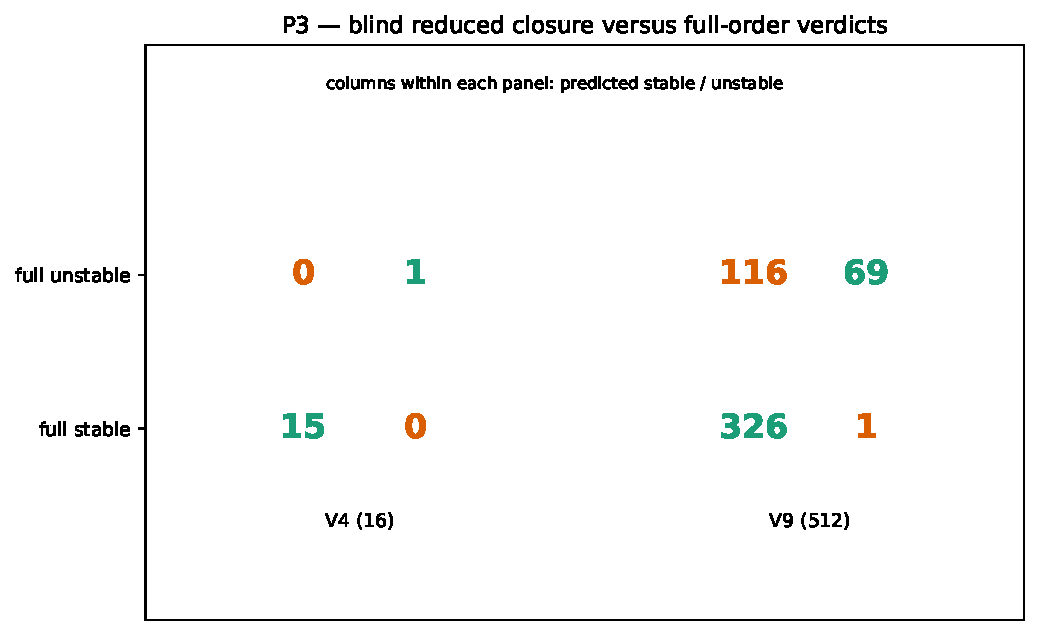
\includegraphics[width=.82\linewidth]{../figures/tx4_blind_prediction/P3_blind_vs_full.pdf}
\caption{Blind reduced closure versus full-order verdicts.}
\end{figure}

\section{Full-order reveal}
V9 truth has 327 stable and 185 unstable cases. The reduced predictor gives
395/512 correct, 116 false-safe, one false-unstable, incorrect H, and exact
minimum blocker cardinality 4. The V4 BASE comparison row was restored from
the frozen FC01 reference because the PCV02 core table omitted BASE; no
prediction was changed.

\section{Controller boundary}
The reduced-only reproduction gives $g_{\rm return}=0.20768138607$ and
0.706424783 Hz. The frozen full-order boundary is
$g_{\rm full}=0.20768140519$; difference $1.91\,10^{-8}$. The reduced search
ran after reveal, so this is not reported as a strict blind boundary claim.

\section{Contextual return}
For $R=H\setminus\{i\}$,
$G_R=(I+Q_{RR})^{-1}$ and
$\mathcal R_{i|R}=Q_{iR}G_RQ_{Ri}$. Classical block algebra gives
\[
\det(I+Q_H)=\det(I+Q_{RR})\det(I-\mathcal R_{i|R}).
\]
The nearest return eigenvalue is $-0.9999999649-5.1\,10^{-9}j$ and maximum
Schur residual is $3.44\,10^{-16}$.
\section{Numerical return validation}
The nine-case audit with three finite-difference factors produced 27 rows.
NumPy and SciPy eigensolvers agreed to displayed precision. Maximum
equilibrium algebraic residual was $1.30\,10^{-12}$. A valid descriptor
$E,A$ pair was not exposed and remains NOT AVAILABLE. The return derivative
check at $a=g$ has maximum error $7.20\,10^{-6}$.

\section{Minimality separation}
\begin{center}
\begin{tabular}{lrrrl}
\toprule
retained GFL buses & missing & $\alpha$ & Hz & verdict\\
\midrule
30+33+35 & 37 & -0.204688 & 0.916019 & stable\\
30+33+37 & 35 & -0.175508 & 0.918500 & stable\\
30+35+37 & 33 & -0.167856 & 0.914639 & stable\\
33+35+37 & 30 & -0.203009 & 0.917627 & stable\\
30+33+35+37 & -- & +0.127006 & 0.622280 & unstable\\
\bottomrule
\end{tabular}
\end{center}
All fifteen proper subsets pass the stable test at P4.

\section{Local versus collective failure}
The proper-subset separation is $\eta_H=0.120831$ in the archived
realization; collective $\sigma_{\min}=2.24\,10^{-8}$. The reduced boundary
run has local $\sigma_{\min}=0.489$ and local determinant minimum 0.433.
This supports collective closure failure, not a local singularity.

\section{Fifteen proper subsets}
The complete finite certificate is
\texttt{results/TX4\_15\_PROPER\_SUBSETS.csv}. BASE, singles, pairs, triples,
and H4 are retained with closure diagnostics.

\section{V9 512-portfolio benchmark}
The V9 result is a negative scalability result: 77.1484 percent accuracy,
116 false-safe cases, one false-unstable case, incorrect H recovery, and
exact kappa recovery. It prevents the phrase 'general exact portfolio
predictor.'

\section{Runtime}
\begin{center}
\begin{tabular}{lrrr}
\toprule
set & full seconds & reduced seconds & full/reduced\\
\midrule
V4, 16 & 2.397 & 4.360 & 0.550\\
V9, 512 & 72.490 & 309.649 & 0.234\\
\bottomrule
\end{tabular}
\end{center}
The reduced method is slower on this hardware.

\section{Aggregate MW/MVA counterexample}
The fixed rule found six-replacement portfolios with normalized mismatch
0.2513 percent; one is unstable ($\alpha=+324.249$) and one stable
($\alpha=-0.1664$). There is no exact aggregate match under the frozen
tolerance. This is supporting evidence, not an exact same-MW/MVA claim.

\section{Lower-order screens}
Singleton, pair, and triple screens pass while H4 fails. H4 lower-order
alpha values are B3 -0.203249, B4 -0.212867, B5 -0.210389, and B5b
-0.183673, all predicting stable H4. Exact reduced closure predicts
unstable. Third-order alpha and determinant truncation remain separate.

\section{Controller remediation}
Changing only $g$ from 0.03625 to fixed validated point 0.25 changes H4 from
$+0.127006$ to $-0.017385\,{\rm s}^{-1}$. This is not an economic optimum.

\section{Nonlinear TDS}
The frozen common disturbance is a +2 percent active-load pulse at bus 20
for 0.2 s. Proper 30+33+35 is stable, H4 at P4 is unstable, and H4 at
$g=0.25$ is stable. All growth signs agree with linear alpha; maximum
primary exponent error is $3.51\,10^{-4}\,{\rm s}^{-1}$. This is phasor
domain TDS, not EMT.

\begin{figure}[ht]
\centering
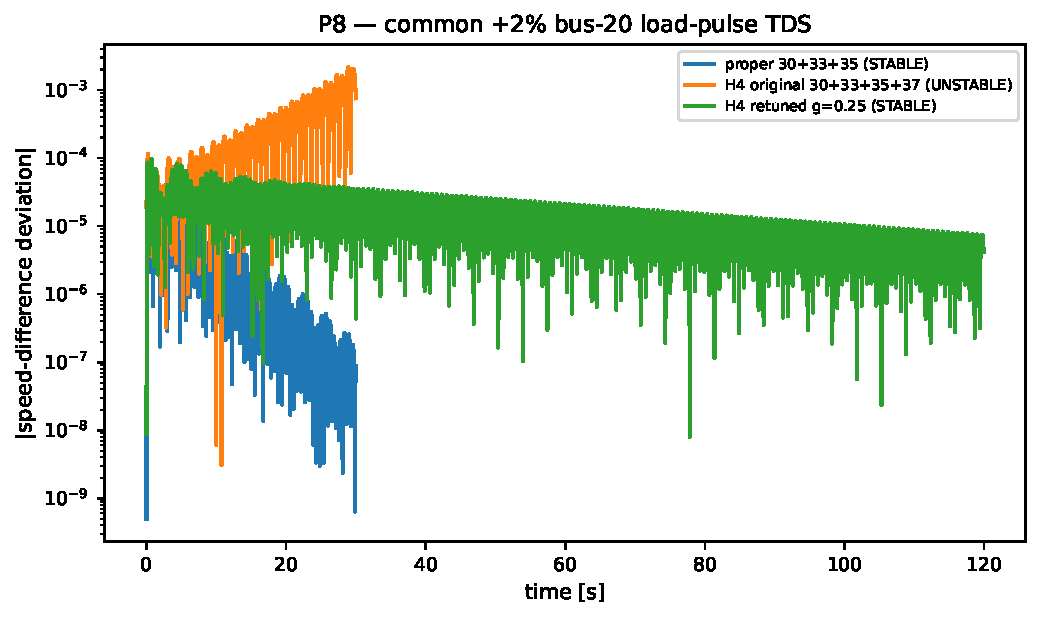
\includegraphics[width=.88\linewidth]{../figures/tx4_blind_prediction/P8_TDS_final.pdf}
\caption{Common-disturbance nonlinear phasor-domain TDS.}
\end{figure}

\section{ANDES}
Existing E31 ANDES results were reused without retuning. They provide
limited independent phasor support for base and selected portfolio
comparisons. Custom-GFL boundary reproduction is NOT TESTED.

\section{EMT status}
EMT portfolio validation is unresolved and no EMT claim is made.

\section{Literature novelty}
The focused audit found extensive prior work on grid strength, impedance and
return ratios, controller stability regions, and IBR planning. It did not
identify in the checked sources the exact combination of finite SG-to-GFL
minimality, pre-reveal reduced prediction, and contextual return conditioned
on remaining devices. This is a scoped distinction, not a priority claim.

\section{Limitations}
One IEEE-39 phasor-domain model, one custom GFL implementation, no EMT
portfolio validation, limited ANDES equivalence, failed V9 H recovery,
slower reduced runtime, and post-reveal timing for the g-boundary search.
No universal or probabilistic claim is allowed.

\section{Reviewer assessments}
Reviewer 1 scores: novelty 7, correctness 8, model adequacy 6, evidence 8,
usefulness 7, IAS impact 8, TPWRS readiness 5. Reviewer 2 scores: novelty 7,
correctness 8, model adequacy 5, evidence 7, usefulness 7, IAS impact 8,
TPWRS readiness 4. Both recommend CASE B poster use with limitations.

\section{IAS poster verdict}
The recommended title is \emph{SAFE ALONE, UNSAFE TOGETHER}. The poster can
show the V4 blind prediction, contextual return, g-only repair, and TDS, but
must show V9 and the boundary timing deviation.

\section{Transactions path}
The package is IAS-ready under a limited predictive claim and not TPWRS-ready.
All artifacts are on the branch
\url{research/tx4-blind-portfolio-prediction-final}; no push was made.

\end{document}
